%----------------------------------------------------------------------------------------
%	PACKAGES AND OTHER DOCUMENT CONFIGURATIONS
%----------------------------------------------------------------------------------------

\documentclass[
	10pt, % Default font size, can be between 8pt and 12pt
]{FreemanCV}


% Handle images:
\graphicspath{{./images/}}


\columnratio{0.50, 0.50} % Widths of the two columns, specified here as a ratio summing to 1 to correspond to percentages; adjust as needed for your content 

% Headers and footers can be added with the following commands: \lhead{}, \rhead{}, \lfoot{} and \rfoot{}
% Example right footer:
%\rfoot{\textcolor{headings}{\sffamily Last update: \today. Typeset with Xe\LaTeX}}

%----------------------------------------------------------------------------------------

\begin{document}

\begin{paracol}{2} % Begin two-column mode

%----------------------------------------------------------------------------------------
%	YOUR NAME AND CURRICULUM VITAE TITLE
%----------------------------------------------------------------------------------------

\parbox[][0.05\textheight][c]{\linewidth}{ % Box to hold your name and CV title; change the fixed height as needed to match the colored box to the right
	\centering % Horizontally center text
	
	{\sffamily\Huge Josh \textbf{Booth}} % Your name
	
	\medskip % Vertical whitespace
	
	%{\cursivefont\Huge\textcolor{headings}{Big Bad Baller}}
	
	\vfill % Push content to the top of the box
}

%----------------------------------------------------------------------------------------
%	MAJOR RESEARCH PROJECT
%----------------------------------------------------------------------------------------

% \section{Doctral Resoearch}

% {\raggedright\textbf{``Observation of Einstein-Podolsky-Rosen Entanglement on Supraquantum Structures by Induction Through Nonlinear Transuranic Crystal of Extremely Long Wavelength Pulse from Mode-Locked Source Array"}\par}

% \medskip % Vertical whitespace

% My research examined the use of ELW pulses from a mode-locked source array inducted through transuranic crystals to observe entanglement on supraquantum structures. Theoretical advancements included prediction of quantum resonance phenomena including the possibility of resonance cascades. I was motivated to conduct this doctoral research due to my passion for teleportation of matter and I believe I have laid the foundation for further experimental validation and development of practical outcomes.

% \medskip % Extra vertical whitespace before the next section

%----------------------------------------------------------------------------------------
%	WORK EXPERIENCE
%----------------------------------------------------------------------------------------

\section{Work Experience}

% Each job is added with a \jobentry command. Below is an empty one to use as a template:

%\jobentry
%	{} % Duration
%	{} % FT/PT (full time or part time)
%	{} % Employer
%	{} % Job title
%	{} % Description

% All 5 parameters must be supplied but any can be empty if you don't need them

%------------------------------------------------

\jobentry
	{Current, from Jun 2022} % Duration
	{FT} % FT/PT (full time or part time)
	{Microchip Technology} % Employer
	{Technical Marketing Engineer} % Job title
	{Developed marketing material and messaging for microcontrollers full go-to-market strategies for 3 products, and } % Description

%------------------------------------------------

\jobentry
	{Feb 1991 -- Jan 1995} % Duration
	{FT} % FT/PT (full time or part time)
	{Black Mesa Research Facility} % Employer
	{Level 3 Research Associate} % Job title
	{This position involved transitioning from purely theoretical work to experimental applications utilising the immense resources of Black Mesa. The transition required an initial learning curve in hazard containment, health and safety procedures and operating experimental infrastructure. Manipulating valves, carts, buttons, levers, etc considerably increased my physical fitness.} % Description

%------------------------------------------------

\jobentry
	{Jul 1982 -- Dec 1984} % Duration
	{PT} % FT/PT (full time or part time)
	{WashPests Limited} % Employer
	{Pest Control Technician} % Job title
	{In this summer job I was tasked with helping eradicate pests from industrial areas. Work involved setting traps, spraying and physical eradication. I received praise for reaching difficult areas and my innovative use of a crowbar to assist in my work.} % Description

%----------------------------------------------------------------------------------------
%	REFERENCES
%----------------------------------------------------------------------------------------

% \section{References}

% %\textit{References available on request} % Uncomment if you'd rather not include references and remove the section below

% %------------------------------------------------

% % This section is laid out using a table. A \tableentry command adds lines with the following parameters:

% %\tableentry{Heading}{Content}{spaceafter}
% % All 3 parameters must be supplied but any can be empty if you don't need them
% % A "spaceafter" value in the third parameter will add some vertical space -- this is to be used between headings, leave it empty for no extra space

% %------------------------------------------------

% \begin{supertabular}{r l} % Start a table with two columns, the table will ensure everything is aligned
	
% 	%------------------------------------------------
	
% 	\tableentry{}{\textbf{Dr. Isaac Kleiner}}{spaceafter}
% 	\tableentry{Position}{Professor}{}
% 	\tableentry{Employer}{\href{https://web.mit.edu/physics/}{Department of Physics}}{}
% 	\tableentry{}{\href{https://web.mit.edu}{\textit{Massachusetts Institute of Technology}}}{spaceafter}
% 	\tableentry{Phone}{+1 (617) 253 1000 x5322 (Work)}{}
% 	\tableentry{Mobile}{+1 (232) 842-3583}{}
	
% 	%------------------------------------------------
	
% 	\\ % Additional vertical whitespace between the references
	
% 	%------------------------------------------------
	
% 	\tableentry{}{\textbf{Dr. Eli Vance}}{spaceafter}
% 	\tableentry{Position}{Scientist (HL1)}{}
% 	\tableentry{Employer}{\href{http://www.bmrf.us}{Black Mesa Research Facility}}{spaceafter}
% 	\tableentry{Email}{\href{mailto:e.vance@bmrf.us}{e.vance@bmrf.us}}{}
% 	\tableentry{Phone}{+1 (800) 786-1410 x6235 (Work)}{}
% 	\tableentry{Mobile}{+1 (201) 632-3901}{}
	
% 	%------------------------------------------------
	
% \end{supertabular}

% \medskip % Extra vertical whitespace before the next section

% %----------------------------------------------------------------------------------------

\switchcolumn % Switch to the second (right) column

%----------------------------------------------------------------------------------------
%	COLORED CONTACT DETAILS BOX
%----------------------------------------------------------------------------------------

\parbox[top][0.1\textheight][c]{\linewidth}{ % Box to hold the colored box; change the fixed height as needed to match the box to the left
	\colorbox{shade}{ % Create colored box and specify background color
		\begin{supertabular}{@{\hspace{3pt}} p{0.05\linewidth} | p{0.775\linewidth}} % Start a table with two columns, the table will ensure everything is aligned
			\raisebox{-1pt}{\faHome} & Chandler, AZ \\ % Address
			\raisebox{-1pt}{\faPhone} & (717) 494-6466 \\ % Phone number
			\raisebox{-1pt}{\small\faEnvelope} & \href{mailto:boothjmail@gmail.com}{boothjmail@gmail.com} \\ % Email address
			\raisebox{-1pt}{\small\faLink} & \href{https://joshbooth.us}{joshbooth.us} \\ % Website
			%\raisebox{-1pt}{\faGithub} & \href{https://github.com/username}{https://github.com/username} \\ % GitHub profile
			%\raisebox{-1pt}{\faLinkedinSquare} & \href{https://www.linkedin.com/in/username}{https://www.linkedin.com/in/username} \\ % LinkedIn profile
			% See fontawesome.pdf in the Fonts folder for all icons you can use
		\end{supertabular}
	}
	\vfill % Push content to the top of the box
}


%----------------------------------------------------------------------------------------
%	ENGINEERING PROJECTS
%----------------------------------------------------------------------------------------

\section{Notable Projects}

\subsection{DMX Light Show}

I believe in action over long-winded discussions. I listen to everyone's viewpoints and use my judgement to immediately act based on consensus to achieve goals quickly and efficiently.



% Entry 1

\setlength\intextsep{20pt} % how far image is down from section title
\begin{wrapfigure}{rt}{0.05\textwidth}
	\hspace*{-20pt} % how close horizontal text can be
    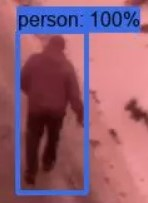
\includegraphics[scale=0.6]{security_system} %Z how large image is
\end{wrapfigure}

\vspace{-15pt} % move image's anchor box up closer to title
\leavevmode\subsection{AI-Driven Security System}

% \begin{figure}[h]
% 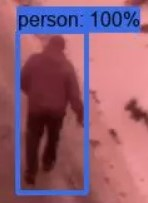
\includegraphics[scale=0.6]{security_system}
% \end{figure}

Manual manipulation of experimental equipment and training within Black Mesa (e.g. the Hazard Course) have contributed to an enjoyment of working with my hands.

\subsection{3D PEEK Printer}

I have been interested in theoretical physics such as quantum mechanics and relativity from an early age. My education and research have cemented this interest into a passion. I greatly enjoy carrying out fundamental physics research with potential practical applications.

\subsection{The Cold Plate}

The cold Plate


%----------------------------------------------------------------------------------------
%	EDUCATION
%----------------------------------------------------------------------------------------

\section{Education} 

% Each qualification entry is added with a \qualificationentry command. Below is an empty one to use as a template:

%\qualificationentry
%	{} % Duration
%	{} % Degree
%	{} % Honors, achievements or distinctions (e.g. first class honors)
%	{} % Department
%	{} % Institution

% All 5 parameters must be supplied but any can be empty if you don't need them

%------------------------------------------------

\begin{supertabular}{r l} % Start a table with two columns, the table will ensure everything is aligned

	%------------------------------------------------
	
	\qualificationentry
		{2018-2022} % Duration
		{Computer Engineering} % Degree
		{Summa Cum Laude; 3.98 GPA} % Honors, achievements or distinctions (e.g. first class honors)
		{Bachelors of Science} % Department
		{Shippensburg University of Pennsylvania} % Institution
	
	%------------------------------------------------
	
	\qualificationentry
		{2018-2022} % Duration
		{Mathematics} % Degree
		{} % Honors, achievements or distinctions (e.g. first class honors)
		{Minor} % Department
		{Shippensburg University of Pennsylvania} % Institution
	
	%------------------------------------------------
	

	%------------------------------------------------

\end{supertabular}

%----------------------------------------------------------------------------------------
%	AWARDS
%----------------------------------------------------------------------------------------

\section{Awards}

% This section is laid out using a table. A \tableentry command adds lines with the following parameters:

%\tableentry{Heading}{Content}{spaceafter}
% All 3 parameters must be supplied but any can be empty if you don't need them
% A "spaceafter" value in the third parameter will add some vertical space -- this is to be used between headings, leave it empty for no extra space

%------------------------------------------------

\begin{supertabular}{r l} % Start a table with two columns, the table will ensure everything is aligned
	
	%------------------------------------------------
	
	\tableentry{1985}{\textbf{Faculty of Science Masters Scholarship}}{}
	\tableentry{}{\textit{Massachusetts Institute of Technology}}{spaceafter}
	
	%------------------------------------------------
	
	\tableentry{1983}{\textbf{Top Achiever Award -- Physics}}{}
	\tableentry{}{\textit{The University of Washington}}{spaceafter}
	
	%------------------------------------------------
	
\end{supertabular}

%----------------------------------------------------------------------------------------
%	COMPUTER SKILLS
%----------------------------------------------------------------------------------------
\section{Testing}
\begin{supertabular}{r l} % Start a table with two columns, the table will ensure everything is aligned
	
	%------------------------------------------------
	
	\tableentry{AI-driven Security System}{\textbf{Faculty of Science Masters Scholarship}}{}
	\tableentry{Manual manipulation of experimental equipment and training within Black Mesa (e.g. the Hazard Course) have contributed to an enjoyment of working with my hands.
}{}
	
\end{supertabular}
% \section{Misc. Skills} 

% % This section is laid out using a table. A \tableentry command adds lines with the following parameters:

% %\tableentry{Heading}{Content}{spaceafter}
% % All 3 parameters must be supplied but any can be empty if you don't need them
% % A "spaceafter" value in the third parameter will add some vertical space -- this is to be used between headings, leave it empty for no extra space

% %------------------------------------------------

% \begin{supertabular}{r l} % Start a table with two columns, the table will ensure everything is aligned
	
% 	%------------------------------------------------
	
% 	\tableentry{Beginner}{Java, MS DOS}{spaceafter}
	
% 	%------------------------------------------------
	
% 	\tableentry{Intermediate}{Javascript, Python, HTML, CSS,}{}
% 	\tableentry{}{Microsoft Windows}{}
% 	\tableentry{}{Computer Hardware \& Support}{spaceafter}
	
% 	%------------------------------------------------
	
% 	\tableentry{Expert}{Perl, Unix, \LaTeX}{spaceafter}
	
% 	%------------------------------------------------
	
% \end{supertabular}

%----------------------------------------------------------------------------------------
%	COMMUNICATION SKILLS
%----------------------------------------------------------------------------------------

% \section{Communication Skills}

% % This section is laid out using a table. A \tableentry command adds lines with the following parameters:

% %\tableentry{Heading}{Content}{spaceafter}
% % All 3 parameters must be supplied but any can be empty if you don't need them
% % A "spaceafter" value in the third parameter will add some vertical space -- this is to be used between headings, leave it empty for no extra space

% %------------------------------------------------

% \begin{supertabular}{r l} % Start a table with two columns, the table will ensure everything is aligned
	
% 	%------------------------------------------------
	
% 	\tableentry{Conferences}{Oral Presentation at the Annual MIT}{}
% 	\tableentry{}{Theoretical Physics Conference -- 1987}{spaceafter}
	
% 	%------------------------------------------------
	
% 	\tableentry{Posters}{Poster at the Meeting of the American}{}
% 	\tableentry{}{Physical Society -- 1985}{spaceafter}
	
% 	%------------------------------------------------
	
% \end{supertabular}


%----------------------------------------------------------------------------------------
%	PUBLICATIONS
%----------------------------------------------------------------------------------------

% \section{Publications}

% %------------------------------------------------

% \textbf{Freeman, G. R.} (1996). Chemistry of Multiply Charged Negative Molecular Ions and Clusters in the Gas Phase:  Terrestrial and in Intense Galactic Magnetic Fields. \textit{The Journal of Physical Chemistry}, \textit{100}(11), 4331-4338.

% \medskip % Vertical whitespace

% Jacobsen, F. M., Gee, N., \textbf{Freeman, G. R.} (1986). Electron mobility in liquid krypton as function of density, temperature, and electric field strength. \textit{Physical Review A}, \textit{34}(3): 2329-2335.

% \medskip % Vertical whitespace

%------------------------------------------------

% As an alternative to a long-form publication list, you can create a shorter summary using only DOI values and years.

% Example \doipublication{} command to add another publication:

%\doipublication{Year}{DOI}{firstauthor}{spaceafter}

% All four parameters are required (can be empty though)
% A value of "firstauthor" in the third parameter will output the DOI in bold
% A "spaceafter" value in the fourth parameter will add some vertical space -- this is to be used between years

%------------------------------------------------

% \subsection{Publications by DOI}

% \begin{supertabular}{r l} % Start a table with two columns, the table will ensure everything is aligned
	
% 	%------------------------------------------------
	
% 	\doipublication{1996}{10.1021/jp951483+}{firstauthor}{spaceafter}
	
% 	%------------------------------------------------
	
% 	\doipublication{1990}{10.1139/p90-097}{firstauthor}{spaceafter}
	
% 	%------------------------------------------------
	
% 	\doipublication{1986}{10.1139/v86-297}{}{}
% 	\doipublication{}{10.1103/PhysRevA.34.2329}{}{spaceafter}
	
% 	%------------------------------------------------
	
% 	& \textit{First author publications in} \textbf{bold}\\
	
% 	%------------------------------------------------
	
% \end{supertabular}

\medskip % Extra whitespace before the next section

%----------------------------------------------------------------------------------------

\end{paracol} % End two-column mode

%----------------------------------------------------------------------------------------

\end{document}
